\documentclass[12pt,a4paper]{article}

\usepackage[utf8]{inputenc}
\usepackage[T1]{fontenc}
\usepackage{lmodern}
\usepackage[a4paper,margin=1in]{geometry}
\usepackage{setspace}
\usepackage{titlesec}
\usepackage{booktabs}
\usepackage{longtable}
\usepackage{array}
\usepackage{xcolor}
\usepackage{hyperref}
\usepackage{fancyhdr}
\usepackage{graphicx}
\usepackage{tocloft}
\usepackage{tikz}
\usetikzlibrary{arrows.meta,positioning,shapes.geometric}

\hypersetup{
  colorlinks=true,
  linkcolor=blue,
  urlcolor=blue,
  citecolor=blue,
  pdftitle={SDLC Project Report - WearBefore},
  pdfauthor={Mohammd Tamim Hossen and Team}
}

\titleformat{\section}{\large\bfseries}{\thesection}{0.6em}{}
\titleformat{\subsection}{\normalsize\bfseries}{\thesubsection}{0.6em}{}

% Table of contents leaders as underscores
\renewcommand{\cftdot}{\textunderscore}
\renewcommand{\cftdotsep}{1.2}
\renewcommand{\cftsecleader}{\cftdotfill{\cftdotsep}}
\renewcommand{\cftsubsecleader}{\cftdotfill{\cftdotsep}}

\setstretch{1.15}
\setlength{\parskip}{0.5em}
\setlength{\parindent}{0pt}
\setlength{\headheight}{14.5pt}

\pagestyle{fancy}
\fancyhf{}
\lhead{WearBefore SDLC Report}
\rhead{\thepage}

\begin{document}

\begin{titlepage}
    \centering
    \vspace*{2cm}
    {\LARGE\bfseries Software Development Life Cycle (SDLC) Project Report\par}
    \vspace{0.8cm}
    {\Large\bfseries WearBefore Fashion E-Commerce Platform\par}
    \vspace{1.2cm}
    {\large Academic/Professional Project Documentation\par}
    \vspace{2cm}

    \begin{tabular}{p{0.28\textwidth} p{0.65\textwidth}}
        \textbf{Project Lead:} & Mohammd Tamim Hossen \\
        \textbf{Project Type:} & Full-Stack Web Application \\
        \textbf{Methodology:} & SDLC (Hybrid Agile-Iterative) \\
        \textbf{Date:} & April 2026 \\
        \textbf{Project Team:} & Mohammd Tamim Hossen (Project Lead), Md Emon Sarkar (Technical Lead), Showrov Shahriarar (Backend Engineer), Montasir Hasan Peal (UI/UX Designer), Nusrat Jahan (QA Engineer), Nushaiba Kawser Era (DevOps and Release Engineer)
    \end{tabular}

    \vfill
    {\large Submitted by Project Team\par}

\end{titlepage}

\tableofcontents
\newpage

\section{Executive Summary}
This report presents the complete Software Development Life Cycle (SDLC) for the \textbf{WearBefore} project, a modern fashion e-commerce platform built with Next.js, TypeScript, Tailwind CSS, Auth0, Neon PostgreSQL, and AI-assisted product recommendation features.

SDLC stands for \textbf{Software Development Life Cycle}. It is the step-by-step process used to plan, build, test, deploy, and maintain software. This project followed SDLC phases to deliver a scalable, secure, and user-friendly platform with shopping, cart, checkout, account management, order history, and AI trial capabilities.

\section{Project Overview}
\subsection{Project Name}
WearBefore Fashion E-Commerce Platform

\subsection{Project Vision}
To provide a high-performance, AI-assisted online shopping platform for fashion products with a smooth end-to-end customer journey from discovery to checkout and post-order account management.

\subsection{Current Scope and Key Features}
At the current stage, WearBefore delivers a complete online shopping journey. Users can discover products by category and search, open detailed product pages, choose size and color variants, and manage cart items smoothly. The platform also supports a full checkout flow, account dashboard, order history, and wishlist experience. On the backend side, authentication is handled through Auth0, while product, cart, and order persistence is managed in Neon PostgreSQL. An AI Trial interface is included to provide product-aware recommendations and style guidance.

\section{Team Structure and Responsibilities}
\begin{longtable}{p{0.35\textwidth} p{0.28\textwidth} p{0.30\textwidth}}
\toprule
\textbf{Name} & \textbf{Role} & \textbf{Primary Responsibilities} \\
\midrule
Mohammd Tamim Hossen & Project Lead & Planning, scope alignment, final decision making, stakeholder communication \\
Md Emon Sarkar & Technical Lead & System design decisions, code quality standards, architecture oversight \\
Showrov Shahriarar & Backend Engineer & API design, database integration, order/cart services \\
Montasir Hasan Peal & UI/UX Designer & User flows, interface consistency, responsive design strategy \\
Nusrat Jahan & QA Engineer & Test planning, validation, defect reporting and regression checks \\
Nushaiba Kawser Era & DevOps and Release Engineer & Deployment pipeline, environment management, release readiness \\
\bottomrule
\end{longtable}

\section{SDLC Methodology Used}
The project used a \textbf{hybrid SDLC model}: structured phase gates for governance and iterative Agile cycles for feature delivery.

\subsection{Why This Model}
This approach was selected because the project needed both control and flexibility. Structured phase gates helped the team maintain clear documentation, delivery milestones, and accountability, while iterative cycles made it possible to refine the user interface, stabilize integrations, and quickly incorporate feedback from real usage.

\section{Phase 1: Planning}
\subsection{Objectives}
During planning, the team focused on clarifying business goals, defining scope boundaries, estimating timeline and effort, and setting realistic success criteria. At the same time, early technical and organizational risks were identified so that mitigation decisions could be made before implementation began.

\subsection{Planned Deliverables}
The planning stage produced a project charter, a milestone roadmap, a first-pass architecture direction, initial technology decisions, and a responsibility allocation model for the core team.

\subsection{Milestone Timeline}
\begin{tabular}{p{0.24\textwidth} p{0.35\textwidth} p{0.30\textwidth}}
\toprule
\textbf{Milestone} & \textbf{Planned Window} & \textbf{Output} \\
\midrule
Planning \& Feasibility & Week 1 & Scope, constraints, timeline \\
Requirements Finalization & Week 2 & Functional and non-functional requirements \\
Design Completion & Week 3--4 & UI flow, architecture, schema draft \\
Development Sprint Cycles & Week 5--9 & Core features and API integration \\
System Testing \& Fixes & Week 10--11 & Defect resolution and validation \\
Deployment \& Handover & Week 12 & Production rollout and runbook \\
\bottomrule
\end{tabular}

\section{Phase 2: Requirements Analysis}
\subsection{Functional Requirements}
From a functional perspective, the system had to support product browsing, filtering, search, product detail viewing, and cart operations. It also needed authenticated checkout, order placement, and account-level order history. Secure login/logout behavior was required, and the AI Trial module needed to generate recommendations grounded in the catalog context.

\subsection{Non-Functional Requirements}
Non-functional expectations focused on responsiveness across devices, stable and secure session handling, reliable data persistence for authenticated users, clean maintainable modular code, and smooth deployment readiness for Vercel.

\subsection{Stakeholders}
The primary stakeholders included end users, the project lead, the engineering team, and the QA/release team responsible for quality gates and rollout confidence.

\section{Phase 3: Design}
\subsection{System Architecture}
The final architecture follows a practical layered model. The presentation layer is handled by Next.js App Router pages and reusable React components. API routes act as the application layer for products, carts, orders, and AI interactions. Neon PostgreSQL serves as the core data layer for users, products, carts, and orders, while Auth0 provides identity and session management.

\begin{figure}[h!]
\centering
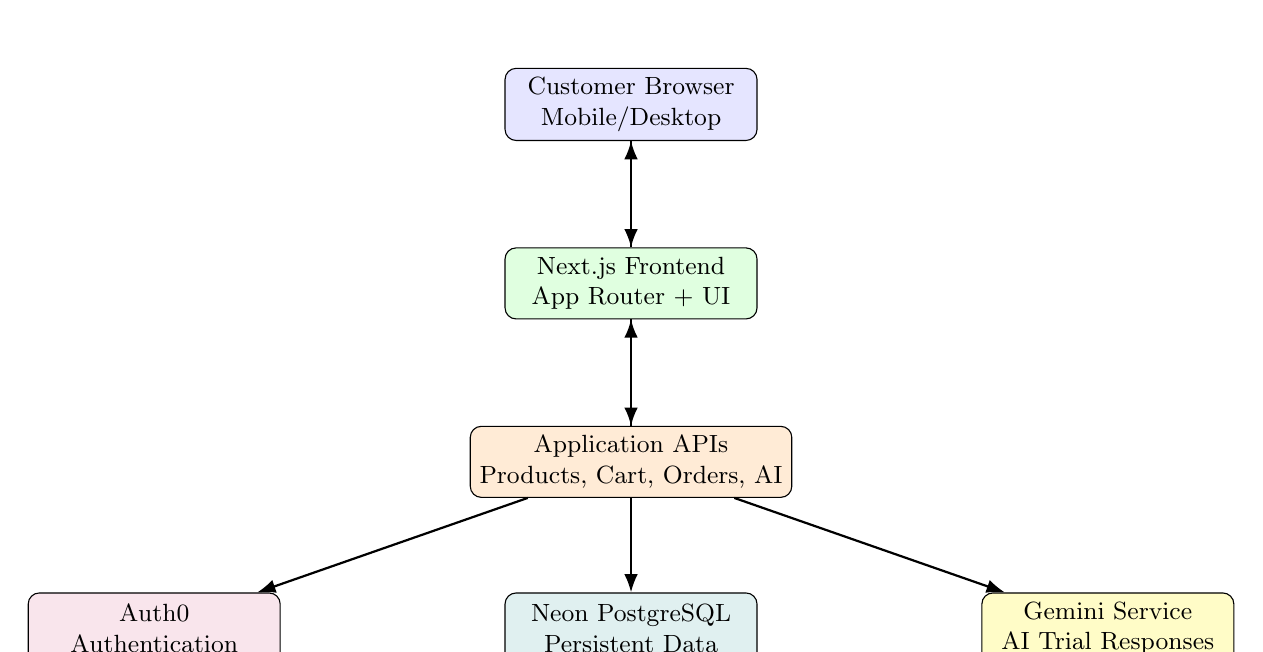
\begin{tikzpicture}[
  node distance=1.35cm and 2.0cm,
  every node/.style={font=\small},
  box/.style={draw, rounded corners, align=center, minimum width=3.2cm, minimum height=0.9cm},
  >=Latex
]
\node[box, fill=blue!10] (user) {Customer Browser\\Mobile/Desktop};
\node[box, fill=green!12, below=of user] (frontend) {Next.js Frontend\\App Router + UI};
\node[box, fill=orange!16, below=of frontend] (api) {Application APIs\\Products, Cart, Orders, AI};
\node[box, fill=purple!10, below left=1.2cm and 2.4cm of api] (auth) {Auth0\\Authentication};
\node[box, fill=teal!12, below=1.2cm of api] (db) {Neon PostgreSQL\\Persistent Data};
\node[box, fill=yellow!22, below right=1.2cm and 2.4cm of api] (ai) {Gemini Service\\AI Trial Responses};

\draw[->, thick] (user) -- (frontend);
\draw[->, thick] (frontend) -- (api);
\draw[->, thick] (api) -- (auth);
\draw[->, thick] (api) -- (db);
\draw[->, thick] (api) -- (ai);
\draw[->, thick, dashed] (api) -- (frontend);
\draw[->, thick, dashed] (frontend) -- (user);
\end{tikzpicture}
\caption{High-level system design of the WearBefore platform}
\label{fig:system-design}
\end{figure}

\subsection{Design Artifacts}
The design work produced an information architecture map, route-level user flows, component and state boundaries, and a database schema covering products, carts, cart items, orders, and order items. API contracts were also documented to align frontend and backend expectations.

\subsection{Technology Design Decisions}
Next.js was selected for its strong routing model and production deployment simplicity. Tailwind CSS enabled fast, consistent UI delivery, while Zustand provided lightweight state management. Auth0 was chosen for secure identity handling, and Neon PostgreSQL was selected for managed relational persistence and predictable data integrity.

\section{Phase 4: Development}
\subsection{Implementation Strategy}
Implementation moved in clear increments. The team first stabilized project foundations such as routing, shared layout, and reusable components. Feature work then progressed through product discovery, cart and checkout behavior, account features, authenticated APIs, and AI Trial integration. This sequence helped reduce rework and kept integration risk under control.

\subsection{Core Stack Used in Implementation}
The production implementation used Next.js 15, React 18, and TypeScript as the foundation; Tailwind CSS and Lucide for interface development; Zustand for client-side state; Auth0 SDK for authentication; and the Neon serverless PostgreSQL driver for database access.

\subsection{Coding Standards and Quality Controls}
Quality controls emphasized type-safe domain models, modular components, predictable API request/response handling, and routine lint and static checks before release candidates were finalized.

\section{Phase 5: Testing}
\subsection{Testing Approach}
A combination of static validation, functional testing, API checks, and manual end-to-end scenario testing was used.

\subsection{Test Coverage Areas}
Testing covered all business-critical flows: authentication lifecycle behavior, protected API access, catalog browsing and filtering, cart state transitions, checkout and order creation, and responsive behavior across common viewport sizes.

\subsection{Sample Test Case Matrix}
\begin{tabular}{p{0.16\textwidth} p{0.48\textwidth} p{0.28\textwidth}}
\toprule
\textbf{Test ID} & \textbf{Scenario} & \textbf{Expected Result} \\
\midrule
TC-01 & Unauthenticated access to cart API & HTTP 401 Unauthorized \\
TC-02 & Login redirect and callback handling & Successful session creation \\
TC-03 & Add/remove/update cart item & Cart state updates correctly \\
TC-04 & Checkout with authenticated user & Order created and persisted \\
TC-05 & View account order history & User sees own orders only \\
TC-06 & Mobile product browsing & Layout remains usable and responsive \\
\bottomrule
\end{tabular}

\section{Phase 6: Deployment}
\subsection{Deployment Strategy}
Deployment followed a release gate process that included production build validation, environment variable verification for Auth0, database, and AI services, and post-deployment smoke testing of login and API health. Vercel was used as the deployment target for stable operational rollout.

\subsection{Release Checklist}
Before each release, the team confirmed that the build passed without blockers, Auth0 callback/logout URLs were correctly configured, database schema and connectivity were healthy, and critical customer journeys worked on the production URL.

\section{Phase 7: Maintenance}
\subsection{Maintenance Objectives}
Maintenance goals are centered on fast defect response, ongoing performance and UX improvements, and incremental feature evolution driven by user behavior and stakeholder priorities.

\subsection{Planned Maintenance Activities}
Planned activities include regular dependency and security updates, structured issue triage from runtime logs, usability refinements for cart/checkout/account flows, and future roadmap items such as payment gateway integration, analytics enrichment, and expanded AI capabilities.

\section{Risk Management}
\begin{tabular}{p{0.34\textwidth} p{0.12\textwidth} p{0.12\textwidth} p{0.34\textwidth}}
\toprule
\textbf{Risk} & \textbf{Prob.} & \textbf{Impact} & \textbf{Mitigation} \\
\midrule
Auth callback misconfiguration & Medium & High & Environment separation and callback URL checklist \\
Third-party API outage & Medium & Medium & Graceful fallback and error handling \\
Schema drift between envs & Low & High & Versioned schema scripts and runtime checks \\
Scope expansion & Medium & Medium & Prioritized backlog and phased delivery \\
\bottomrule
\end{tabular}

\section{Stage-Wise SDLC Deliverables Summary}
\begin{longtable}{p{0.18\textwidth} p{0.74\textwidth}}
\toprule
\textbf{SDLC Stage} & \textbf{Delivered Output} \\
\midrule
Planning & Scope definition, timeline, milestones, role allocation \\
Requirements Analysis & Functional and non-functional requirement baseline \\
Design & Architecture model, route map, API and schema design \\
Development & Feature implementation, integrations, code modularization \\
Testing & Functional validation, access-control checks, defect correction \\
Deployment & Build release, environment setup, production rollout \\
Maintenance & Monitoring, bug fixes, iterative improvements, roadmap updates \\
\bottomrule
\end{longtable}

\section{Conclusion}
The WearBefore project demonstrates an end-to-end SDLC implementation from planning to maintenance. By combining structured SDLC controls with iterative delivery, the team successfully delivered a production-ready e-commerce system with modern authentication, persistent data architecture, and AI-assisted user features.

The process and artifacts in this report can be reused as a template for future full-stack web projects requiring clear governance, practical engineering execution, and continuous post-release improvement.

\section*{Appendix A: SDLC Stage Definitions}
\addcontentsline{toc}{section}{Appendix A: SDLC Stage Definitions}
\textbf{Planning:} define goals, scope, budget, and timeline so the project starts with realistic constraints and shared expectations.\\
\textbf{Requirements Analysis:} gather and clarify what the software must do, including both business behavior and quality expectations.\\
\textbf{Design:} establish architecture, interface direction, data models, and workflow logic before implementation deepens.\\
\textbf{Development:} implement and integrate features in code while following quality standards and review discipline.\\
\textbf{Testing:} detect defects early, verify expected behavior, and confirm reliability across critical scenarios.\\
\textbf{Deployment:} release validated software to production in a controlled and observable way.\\
\textbf{Maintenance:} continue to support users, address incidents, and improve the product over time.

\end{document}
